
\documentclass[10pt]{article}

\usepackage[margin=0.8in]{geometry}
\usepackage[utf8]{inputenc}
\usepackage[T1]{fontenc}
\usepackage[english]{babel}

% --- Font Setup ---
\usepackage{fourier}             % Use the Fourier font (or choose another like lmodern, times, etc.)
\usepackage{amsmath}             % For math formulas
\usepackage{amssymb}             % For math symbols
\usepackage{amsfonts}            % For math fonts
\usepackage{amsthm}              % For theorem environments (if needed)

% --- Graphics and Floats ---
\usepackage{graphicx}            % To include graphics
\usepackage{float}               % For figure placement control (e.g., [H])
\usepackage{caption}             % For better caption control
\usepackage{subcaption}          % For subfigures (if needed)

% --- Tables ---
\usepackage{booktabs}            % For professional looking tables

% --- Utilities and Formatting ---
\usepackage{etoolbox}            % General utility package
\usepackage{siunitx}             % For consistent number and unit formatting (e.g., \num{10000})
\usepackage{parskip}             % Adds space between paragraphs instead of indentation (optional style choice)
\usepackage{hyperref}            % For clickable links (sections, URLs, citations)
\usepackage{cite}                % For improved citation handling

% --- Code Listings (Optional) ---
\usepackage{listings}            % For code snippets
\usepackage{color}               % Required by listings

\definecolor{codegreen}{rgb}{0,0.6,0}
\definecolor{codegray}{rgb}{0.5,0.5,0.5}
\definecolor{codepurple}{rgb}{0.58,0,0.82}
\definecolor{backcolour}{rgb}{0.95,0.95,0.92}

\lstdefinestyle{mystyle}{
    backgroundcolor=\color{backcolour},
    commentstyle=\color{codegreen},
    keywordstyle=\color{magenta},
    numberstyle=\tiny\color{codegray},
    stringstyle=\color{codepurple},
    basicstyle=\ttfamily\footnotesize,
    breakatwhitespace=false,
    breaklines=true,
    captionpos=b,
    keepspaces=true,
    numbers=left,
    numbersep=5pt,
    showspaces=false,
    showstringspaces=false,
    showtabs=false,
    tabsize=2,
    language=C++ % Set default language
}
\lstset{style=mystyle}

% --- Custom Commands ---
\newcommand{\code}[1]{\texttt{#1}} % Helper for inline code formatting

% --- Hyperref Setup ---
\hypersetup{
    colorlinks=true,
    linkcolor=blue,      % Color for internal links (sections, figures)
    citecolor=codegreen, % Color for citations
    urlcolor=cyan,       % Color for URLs
    pdftitle={Assignment 2: Collatz Conjecture Parallelization},
    pdfauthor={Luca Lombardo}, % Replace with your name
    pdfsubject={SPM Course Assignment},
    pdfkeywords={Collatz, C++, Parallel Computing, Threading, Scheduling, Work-Stealing, Lock-Free},
}

% --- Title Information ---
\title{Assignment 2: Parallel Collatz Problem}
\author{Luca Lombardo \\ SPM Course a.a. 24/25} % Replace with your name
\date{} % Use current date, or set a specific one

%==============================================================================
% Document Start
%==============================================================================
\begin{document}

\maketitle
\vspace{-1.5em} % Adjust space after title/author block

% --- Abstract ---
% \begin{abstract}
%   This report presents the parallelization strategies developed for computing maximum Collatz sequence lengths across multiple ranges using C++17 threading primitives. Custom static (Block, Cyclic, Block-Cyclic) and dynamic (initially Centralized Queue, later Lock-Free Work-Stealing) schedulers were implemented. Key design choices focused on minimizing synchronization overhead using atomic operations for result aggregation and exploring scalable dynamic scheduling via a Chase-Lev deque implementation. Challenges related to overflow handling, multi-range static scheduling, and concurrent deque correctness are discussed alongside the rationale for the implemented solutions.
% \end{abstract}

% --- Main Content ---

% \section{Introduction}
% The Collatz conjecture offers a computationally intensive problem suitable for exploring parallel execution strategies. This project focuses on implementing custom parallel schedulers in C++17 to find the maximum Collatz sequence length within user-specified ranges, emphasizing the design choices and trade-offs involved in static versus dynamic load balancing and synchronization techniques. The goal is to compare these custom implementations both theoretically and experimentally. All parallel implementations utilize \code{std::thread} and rely on atomic operations (\code{std::atomic}) for efficient, fine-grained result aggregation from concurrent tasks.

% \section{Core Computation and Parallel Framework}
% The core \code{collatz\_steps} function uses \code{unsigned long long} (\code{ull}) and incorporates overflow detection via pre-computation checks to ensure correctness. The parallel framework divides the input ranges into chunks (tasks). A common challenge is aggregating the maximum step count found for each original range from potentially many concurrently executing tasks. This was addressed using an \code{std::atomic<ull>} counter per range, updated via compare-and-swap (CAS) loops by worker threads upon task completion. This atomic approach avoids coarse-grained locks on results, minimizing synchronization overhead at this stage. Memory ordering (\code{std::memory\_order\_relaxed} for loads, \code{std::memory\_order\_release} for successful stores) was employed to balance performance and correctness. The primary differentiation between parallel implementations lies in the task distribution strategy (scheduling).

\section{Sequential Baseline and Core Function} % NEW CONCISE SECTION
The sequential implementation serves as our reference baseline. The \code{collatz\_steps(ull n)} function ensures correctness using \code{unsigned long long} types and overflow detection. For efficiency we use bitwise operations to handle parity checks and division. A key optimization targets power-of-two inputs ($n=2^k$): rather than iteratively dividing by two $k$ times, the function directly computes the result $k$ using the \code{\_\_builtin\_ctzll} intrinsic (count trailing zeros), significantly accelerating these cases. This implementation processes all input ranges through \code{find\_max\_steps\_in\_subrange}.

\section{Parallel Implementation Framework}
I built parallel versions using \code{std::thread} by partitioning input ranges into smaller tasks (chunks) that worker threads execute concurrently. For thread-safe aggregation of maximum step counts for each original range, I implemented a \code{RangeResult} structure containing \code{std::atomic<ull>} variables. Worker threads update these atomically via compare-and-swap (CAS) loops upon task completion. I chose this fine-grained approach to minimize synchronization bottlenecks during result updates. My implementations differ primarily in their task distribution (scheduling) strategy.

\subsection{Static Scheduling Strategies}
Static scheduling assigns tasks to threads deterministically before execution starts. I implemented three variants to compare their characteristics:
\begin{itemize}
    \item \textbf{Block:} Assigns large contiguous blocks per range to each thread. It features low scheduling overhead but suffers from poor load balancing, especially for non-uniform workloads\footnote{like Collatz where computation cost per number varies significantly.}.
    \item \textbf{Cyclic:} Assigns individual numbers round-robin. Offers fine-grained load balancing but can lead to suboptimal cache performance due to scattered memory accesses.
    \item \textbf{Block-Cyclic:} Divides work into blocks of a specified \code{chunk\_size}, which are then assigned cyclically using a global block index computed across all input ranges. This strategy aims to balance load better than pure Block while potentially improving cache locality compared to pure Cyclic.
\end{itemize}
Static schedulers are typically suitable for predictable, balanced workloads due to their minimal runtime overhead.


\subsection{Dynamic Scheduling Strategies}
For workloads with variable task execution times like Collatz computation, I found dynamic scheduling strategies typically outperform static assignments. Since they let idle threads grab new tasks as they become available, they significantly improve load balancing. I explored three dynamic scheduling approaches:

\begin{enumerate}
    \item \textbf{Centralized Task Queue:} I implemented this straightforward approach using a single shared queue (my \code{TaskQueue} class) protected by a \code{std::mutex} and a \code{std::condition\_variable} to efficiently manage thread signaling. This approach was simple to implement and provided natural load balancing since any free thread could take the next task whenever it became available. However, I quickly discovered a major limitation - the single mutex protecting the queue became a bottleneck with many threads competing for access, limiting scalability as thread count increased. Despite this limitation, I successfully implemented and benchmarked this approach as a baseline for comparison.

    \item \textbf{Work-Stealing with Mutex-Based Deques:} To address the scalability issues in my centralized approach, I decentralized task management by giving each thread its own deque (my \code{WorkStealingQueue} class). Threads primarily work with their local queue (using LIFO operations for better cache locality) but can "steal" tasks (using FIFO operations) from other threads when they become idle. This significantly reduced contention compared to my centralized queue implementation and scaled much better with higher thread counts. The LIFO access pattern for local work also improved cache locality for better performance.

    \item \textbf{Lock-Free Work-Stealing:} Pushing for even better performance, I attempted using exclusively atomic operations and carefully controlled memory ordering to eliminate mutexes entirely. This approach theoretically offers the highest performance by completely avoiding lock contention, but I found it extremely difficult to implement correctly. Managing atomics and memory ordering proved challenging, especially with edge cases like concurrent operations on nearly-empty deques where multiple threads might try to take the last task simultaneously.
\end{enumerate}

I spent considerable time trying to implement a lock-free work-stealing deque based on Chase-Lev principles. Despite focusing on atomic interactions and memory synchronization, my implementation was unstable - it often deadlocked or hung during testing. I noticed its behavior changed with subtle timing variations or even debugging prints, classic signs of complex race conditions. Given these challenges and the project timeframe, I made a practical decision to focus on ensuring robust implementations of the other two approaches. I fully implemented, tested and benchmarked both the Centralized Task Queue and Mutex-Based Work-Stealing approaches for this report.
\section{Theoretical Performance Analysis}

We applied the Work-Span model to estimate the inherent parallelism in the benchmark workloads. Work (W) was approximated as the total Collatz steps across all numbers, and Span (S) as the maximum steps for any single number. The theoretical Parallelism $P = W/S$ indicates the maximum possible speedup, neglecting overheads.

% Use the results you provided earlier
\begin{table}[H] % Use [H] for "here if possible" placement
    \centering
    \caption{Theoretical Work-Span Analysis Results for Benchmark Workloads.}
    \label{tab:theoretical}
    \begin{tabular}{@{}l S[table-format=9.0] S[table-format=3.0] S[table-format=6.1]@{}} % Adjust table formats as needed
        \toprule
        Workload Description                                                      & {Work (W)} & {Span (S)} & {Parallelism (P=W/S)} \\ \midrule
        Medium Balanced (1-100k)                                                  & 10753840   & 350        & 30725.3               \\
        Large Balanced (1-1M)                                                     & 131434424  & 524        & 250829.0              \\
        Unbalanced Mix (Small, Large, Medium)                                     & 66057430   & 448        & 147450.0              \\
        Many Small Uniform Ranges (500x1k)                                        & 62134795   & 448        & 138694.0              \\
        Ranges Around Powers of 2 (2\textasciicircum{}8 to 2\textasciicircum{}20) & 1271514    & 363        & 3502.8                \\
        Extreme Imbalance with Isolated Expensive Calculations                    & 1113876    & 685        & 1626.1                \\ \bottomrule
    \end{tabular}
\end{table}

The results in Table \ref{tab:theoretical} show that theoretical Parallelism ($P$) varies significantly, primarily driven by the large differences in total Work (W) across workloads. Workloads processing substantially more numbers (e.g., "Large Balanced", "Unbalanced Mix") naturally have orders of magnitude more total work. Since the Span (S), determined by the single longest sequence, varies relatively little (within a factor of $\approx$2 in this case), the $P=W/S$ ratio largely mirrors the scale of W.

Therefore, while workloads like "Large Balanced" show extremely high theoretical parallelism ($P \approx 250k$), indicating vast potential for parallel execution limited mainly by processor count, workloads like "Extreme Imbalance" ($P \approx 1.6k$) are theoretically limited sooner, not necessarily because their critical path is intrinsically problematic relative to the type of work, but because the total amount of work (W) is much smaller compared to their Span (S). This suggests that achieving high speedups on smaller workloads might be challenging even theoretically, before considering practical overheads. This idealized analysis provides context for evaluating experimental speedups.
%%%%%%%%%%%%%%%%%%%%%%%%%%%%%%%%%%%%%%%%%%%%%%%%%%%%%%%%%%%%%%%%%%%%%%%%%%%%%%%
% --- Experimental Performance Analysis Section (Complete & Revised) ---
%%%%%%%%%%%%%%%%%%%%%%%%%%%%%%%%%%%%%%%%%%%%%%%%%%%%%%%%%%%%%%%%%%%%%%%%%%%%%%%
\section{Experimental Performance Analysis}

The parallel implementations were benchmarked on a machine equipped with two Intel(R) Xeon(R) Gold 5318Y CPUs. Each CPU has 24 physical cores supporting Hyper-Threading, providing 48 logical threads per socket, for a system total of 48 physical cores and 96 logical threads. This dual-socket configuration presents a Non-Uniform Memory Access (NUMA) architecture, where memory access latency differs depending on whether a thread accesses memory local to its own CPU socket or remote memory attached to the other socket. The system runs Ubuntu 22.04 (Linux kernel 5.15.0-119-generic) and is equipped with 1TB of RAM distributed across the sockets. All code was compiled using GCC 11.4.0 with options \code{-std=c++17 -O3 -pthread}. Execution times reported are the median of 10 samples, each consisting of 50 iterations, to mitigate measurement noise. Strong speedup is calculated relative to the optimized sequential baseline for each workload. Tests varied thread counts up to 96 and chunk sizes from 16 to 1024.

\subsection{Static vs. Dynamic Scheduling Speedup}
The performance comparison between static and dynamic schedulers highlights the importance of workload characteristics and the underlying hardware architecture. Figure \ref{fig:speedup_comparison_grid} presents the speedup achieved on four representative workloads, utilizing the empirically determined optimal chunk size for chunk-dependent schedulers (Dynamic, Static Block-Cyclic) for each specific workload.

\begin{figure}[H]
    \centering
    \begin{subfigure}[b]{0.49\textwidth}
        \centering
        % USE YOUR ACTUAL FILENAME HERE (Workload ID 1 - Large Balanced)
        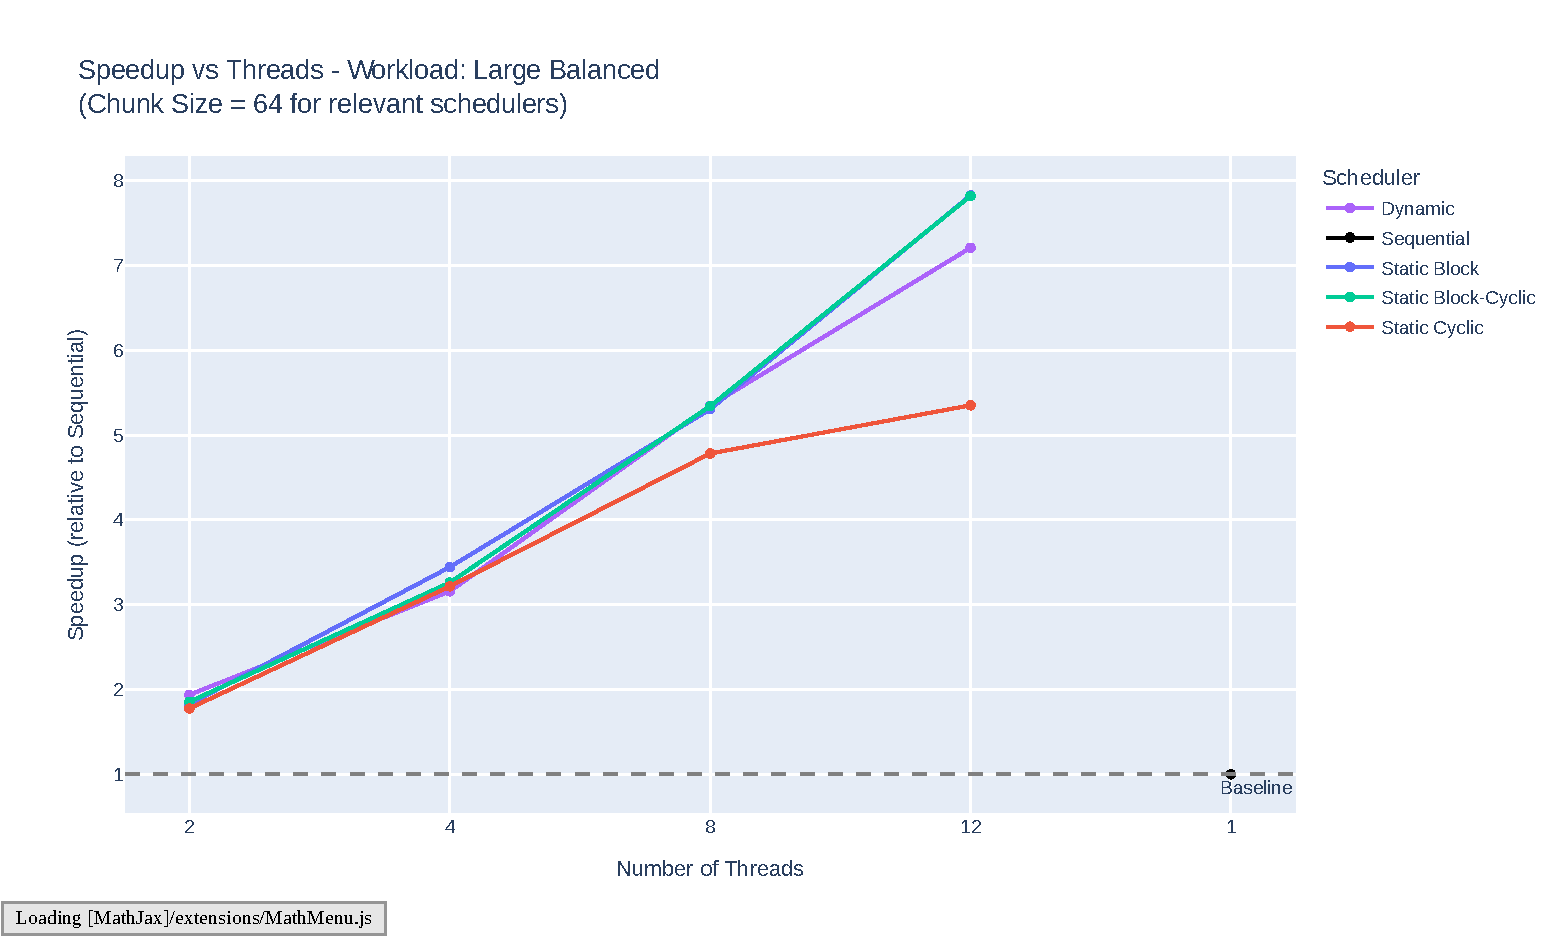
\includegraphics[width=\textwidth]{../results/plots_sencha/speedup_vs_threads/speedup_vs_threads_W1.pdf}
        \caption{Large Balanced (1-1M)}
        \label{fig:speedup_large_balanced}
    \end{subfigure}
    \hfill % Add some horizontal space
    \begin{subfigure}[b]{0.49\textwidth}
        \centering
        % USE YOUR ACTUAL FILENAME HERE (Workload ID 5 - Extreme Imbalance)
        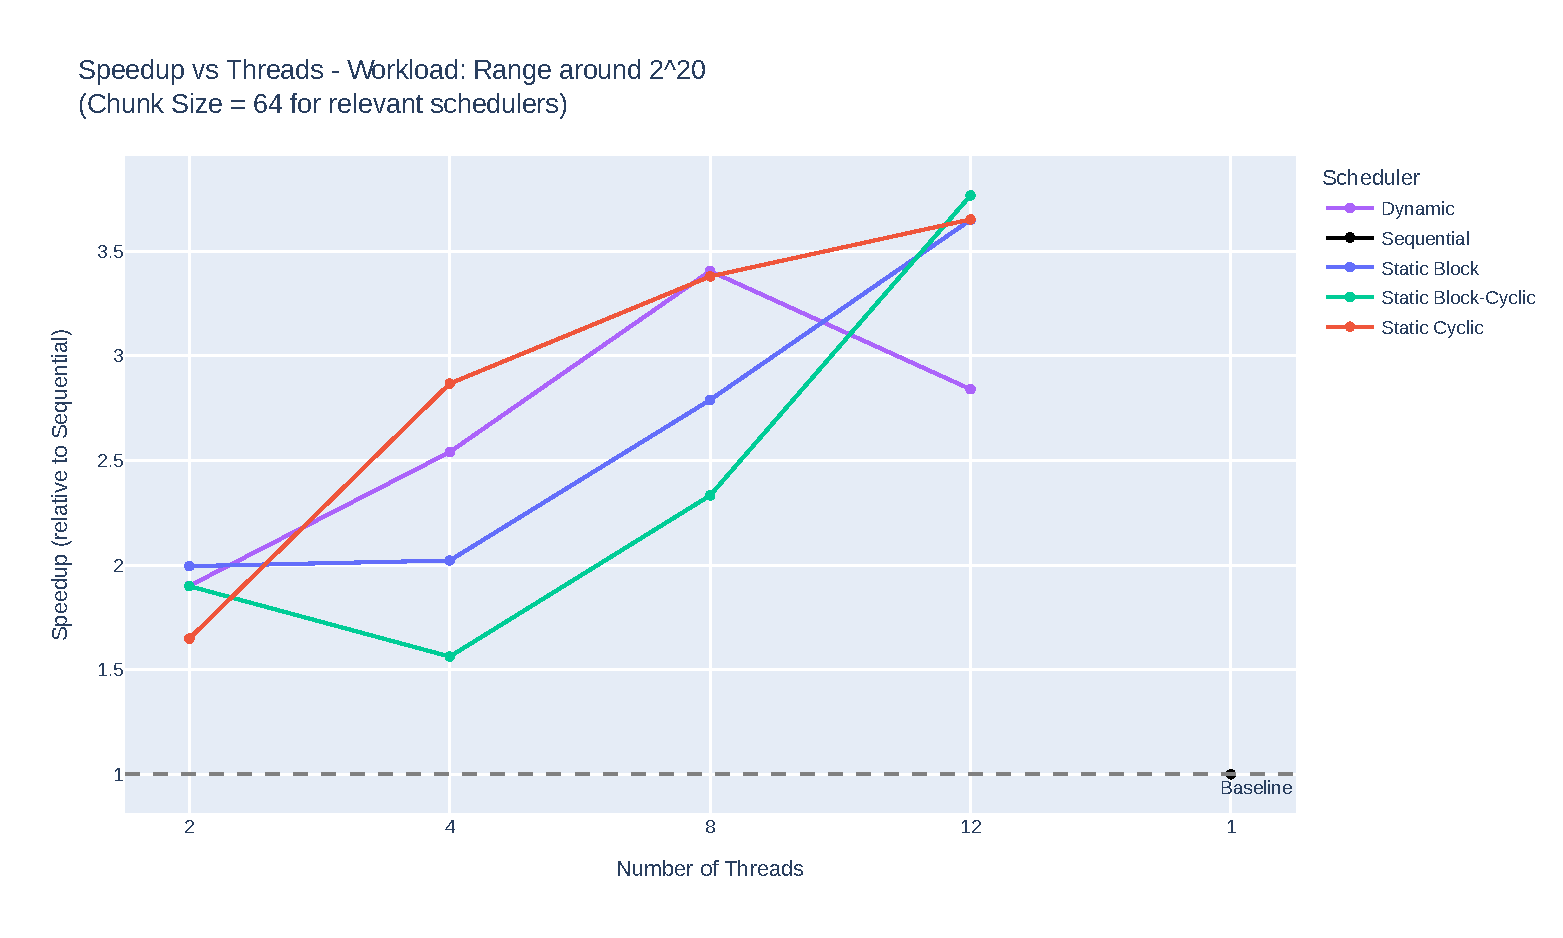
\includegraphics[width=\textwidth]{../results/plots_sencha/speedup_vs_threads/speedup_vs_threads_W5.pdf}
        \caption{Extreme Imbalance}
        \label{fig:speedup_extreme_imbalance}
    \end{subfigure}

    \vspace{1em} % Add some vertical space between rows

    \begin{subfigure}[b]{0.49\textwidth}
        \centering
        % USE YOUR ACTUAL FILENAME HERE (Workload ID 2 - Unbalanced Mix)
        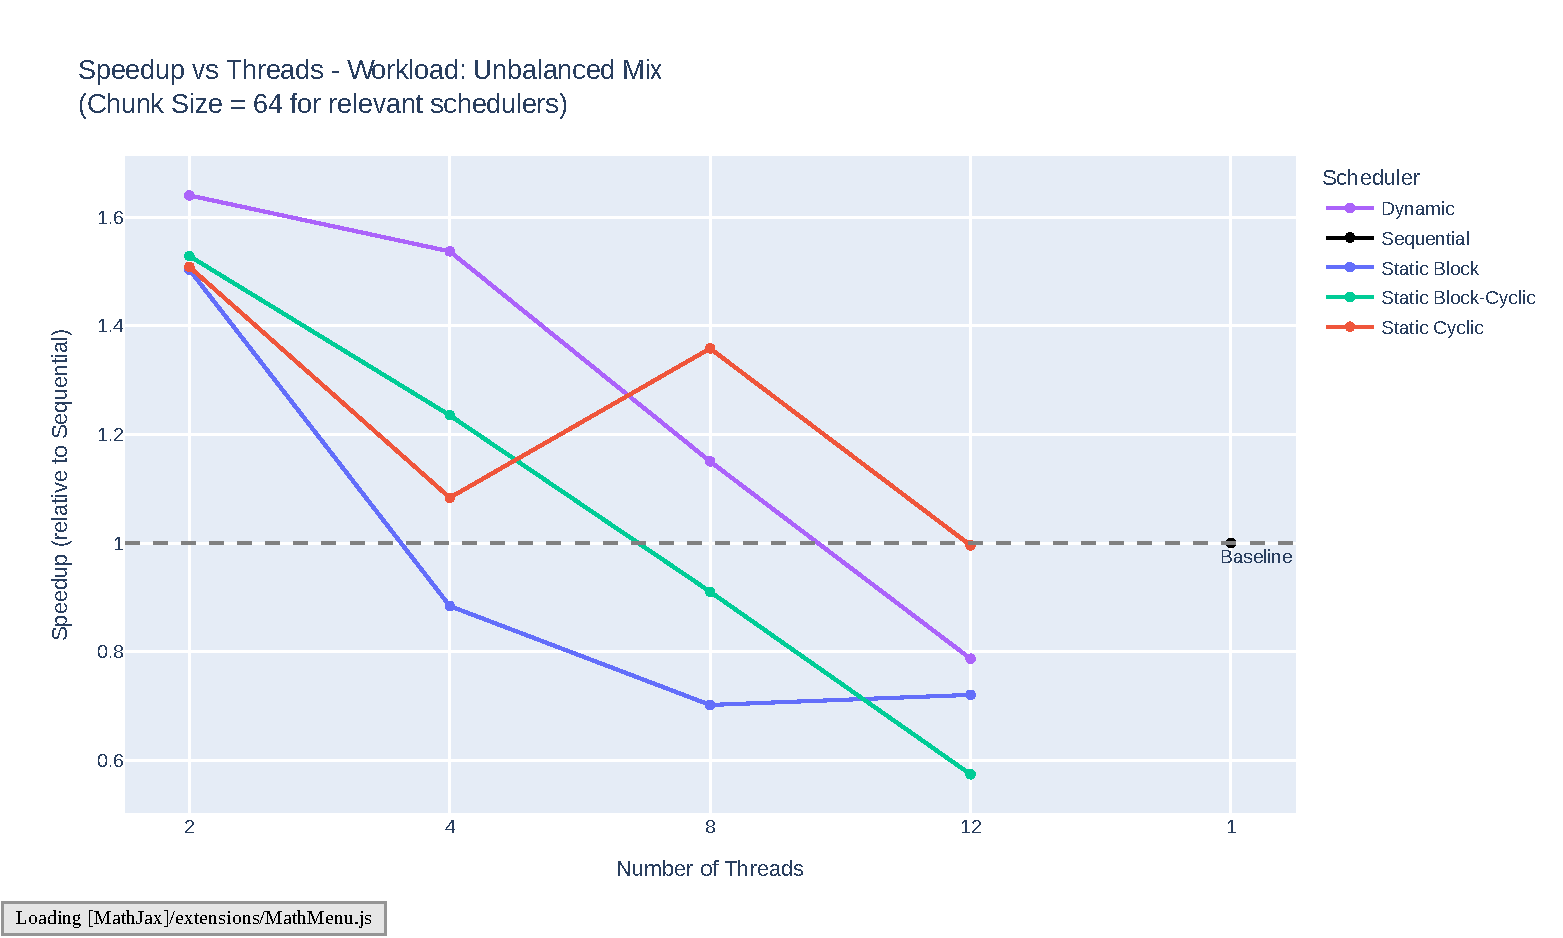
\includegraphics[width=\textwidth]{../results/plots_sencha/speedup_vs_threads/speedup_vs_threads_W2.pdf}
        \caption{Unbalanced Mix (Small, Large, Medium)}
        \label{fig:speedup_unbalanced_mix}
    \end{subfigure}
    \hfill % Add some horizontal space
    \begin{subfigure}[b]{0.49\textwidth}
        \centering
        % USE YOUR ACTUAL FILENAME HERE (Workload ID 3 - Many Small)
        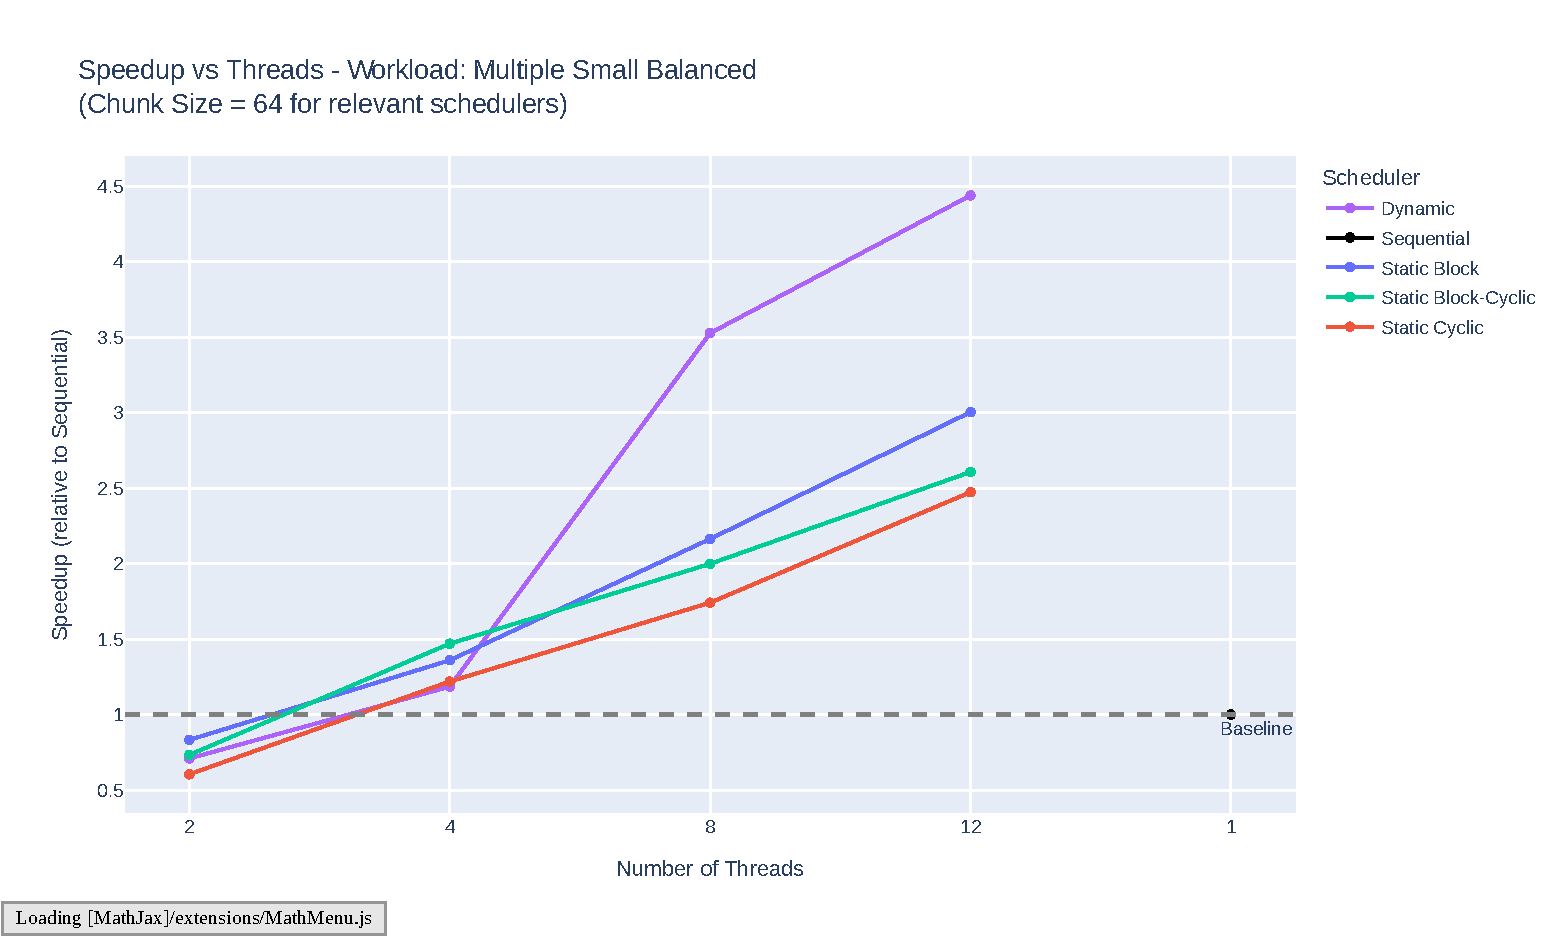
\includegraphics[width=\textwidth]{../results/plots_sencha/speedup_vs_threads/speedup_vs_threads_W3.pdf}
        \caption{Many Small Uniform Ranges (500x1k)}
        \label{fig:speedup_many_small}
    \end{subfigure}

    \caption{Speedup vs. Threads for selected workloads (Schedulers use optimal chunk size per workload). Note varying y-axis scales and performance beyond 48 threads.}
    \label{fig:speedup_comparison_grid}
\end{figure}

For reasonably balanced or mixed workloads (Fig \ref{fig:speedup_large_balanced}, \ref{fig:speedup_unbalanced_mix}, \ref{fig:speedup_many_small}), the dynamic work-stealing scheduler generally achieves the highest peak speedup, often slightly exceeding Static Block-Cyclic when optimally tuned. Both scale well up to roughly the capacity of one CPU socket (48 threads).

However, the "Extreme Imbalance" workload (Fig \ref{fig:speedup_extreme_imbalance}) reveals a striking inversion. The dynamic work-stealing scheduler, expected to excel with imbalance, performs significantly worse than static schedulers (especially Static Block-Cyclic and Cyclic) beyond approximately 16 threads. This suggests that its overhead becomes detrimental when managing tasks with extreme duration variance (with many tasks being near-instantaneous while a few are very long). One potential cause is the high relative overhead, where the cost of lock-free deque operations, such as atomic operations and the maintenance of cache coherence, dominates the execution time for these numerous trivial tasks. Additionally, rapid idling of many threads may lead to concentrated contention or wasted effort when stealing very small tasks. In contrast, static methods, despite their load imbalance, benefit from minimal runtime overhead, which proves advantageous in this specifically highly skewed scenario.

A key observation across all workloads is performance degradation beyond 48 threads (Fig \ref{fig:speedup_large_balanced}). This reflects the system's dual-socket NUMA architecture: when execution spans both sockets, cross-socket communication for shared data structures and cache coherence incurs significant latency. The implemented schedulers are NUMA-unaware, limiting their scalability across multiple sockets.

\subsection{Impact of Chunk Size}
The chunk size parameter is crucial for tuning performance, mediating the trade-off between scheduling overhead (favoring larger chunks) and load balancing granularity (favoring smaller chunks). Figure \ref{fig:chunk_impact} compares the speedup achieved by the Dynamic (Work-Stealing) and Static Block-Cyclic schedulers across various chunk sizes for both the "Large Balanced" and "Extreme Imbalance" workloads.

\begin{figure}[H]
    \centering
    \begin{subfigure}[b]{0.49\textwidth}
        \centering
        % USE YOUR ACTUAL FILENAME HERE (Dynamic W1)
        \includegraphics[width=\textwidth]{../results/plots_sencha/dynamic_chunk_comparison/dynamic_chunks_W1.pdf}
        \caption{Dynamic: Large Balanced (1-1M)}
        \label{fig:chunk_impact_dynamic_balanced}
    \end{subfigure}
    \hfill
    \begin{subfigure}[b]{0.49\textwidth}
        \centering
        % USE YOUR ACTUAL FILENAME HERE (Dynamic W5)
        \includegraphics[width=\textwidth]{../results/plots_sencha/dynamic_chunk_comparison/dynamic_chunks_W5.pdf}
        \caption{Dynamic: Extreme Imbalance}
        \label{fig:chunk_impact_dynamic_imbalance}
    \end{subfigure}

    \vspace{0.5em} % Optional vertical space

    \begin{subfigure}[b]{0.49\textwidth}
        \centering
        % USE YOUR ACTUAL FILENAME HERE (Static BC W1)
        \includegraphics[width=\textwidth]{../results/plots_sencha/static_block_cyclic_chunk_comparison/static_block_cyclic_chunks_W1.pdf}
        \caption{Static Block-Cyclic: Large Balanced (1-1M)}
        \label{fig:chunk_impact_sbc_balanced}
    \end{subfigure}
    \hfill
    \begin{subfigure}[b]{0.49\textwidth}
        \centering
        % USE YOUR ACTUAL FILENAME HERE (Static BC W5)
        \includegraphics[width=\textwidth]{../results/plots_sencha/static_block_cyclic_chunk_comparison/static_block_cyclic_chunks_W5.pdf}
        \caption{Static Block-Cyclic: Extreme Imbalance}
        \label{fig:chunk_impact_sbc_imbalance}
    \end{subfigure}

    \caption{Impact of Chunk Size on Scheduler Speedup vs. Threads for selected workloads.}
    \label{fig:chunk_impact}
\end{figure}

A notable observation is the difference in sensitivity to chunk size. Static Block-Cyclic (Figures \ref{fig:chunk_impact_sbc_balanced}, \ref{fig:chunk_impact_sbc_imbalance}) appears relatively robust, showing similar performance across a wider range of medium-to-large chunk sizes once sufficient threads are active. This is likely because its overhead is primarily fixed per block assignment, regardless of the stealing activity. In contrast, the Dynamic scheduler (Figures \ref{fig:chunk_impact_dynamic_balanced}, \ref{fig:chunk_impact_dynamic_imbalance}) displays stronger workload-dependent sensitivity. For the "Large Balanced" workload, larger chunks (512-1024) perform best, likely minimizing the overhead of deque operations (pushes, pops, steals) when load balancing is less critical. Conversely, for the "Extreme Imbalance" workload, these same large chunks yield poor results; smaller chunks (e.g., 64-256) become necessary, despite their higher overhead, to provide the granularity needed for work-stealing to effectively distribute the highly variable task durations. This highlights that dynamic scheduling requires more careful tuning of task granularity based on workload characteristics to maximize its benefits.

\subsection{Performance Heatmaps}
Heatmaps visualize performance across the thread/chunk size space, confirming the optimal regions. Figures \ref{fig:heatmaps_balanced} and \ref{fig:heatmaps_imbalanced} show these patterns for balanced and imbalanced workloads respectively.

\begin{figure}[H]
    \centering
    \begin{subfigure}[b]{0.49\textwidth}
        \centering
        % USE YOUR ACTUAL FILENAME HERE (Dynamic W1)
        \includegraphics[width=\textwidth]{../results/plots_sencha/speedup_heatmaps_chunk_vs_threads/heatmap_speedup_dynamic_W1.pdf}
        \caption{Dynamic: Large Balanced (1-1M)}
        \label{fig:heatmap_dynamic_balanced}
    \end{subfigure}
    \hfill
    \begin{subfigure}[b]{0.49\textwidth}
        \centering
        % USE YOUR ACTUAL FILENAME HERE (Static BC W1)
        \includegraphics[width=\textwidth]{../results/plots_sencha/speedup_heatmaps_chunk_vs_threads/heatmap_speedup_static_block_cyclic_W1.pdf}
        \caption{Static BC: Large Balanced (1-1M)}
        \label{fig:heatmap_sbc_balanced}
    \end{subfigure}
    \caption{Speedup Heatmaps for Balanced Workload (Chunk Size vs. Number of Threads).}
    \label{fig:heatmaps_balanced}
\end{figure}

\begin{figure}[H]
    \centering
    \begin{subfigure}[b]{0.49\textwidth}
        \centering
        % USE YOUR ACTUAL FILENAME HERE (Dynamic W5)
        \includegraphics[width=\textwidth]{../results/plots_sencha/speedup_heatmaps_chunk_vs_threads/heatmap_speedup_dynamic_W5.pdf}
        \caption{Dynamic: Extreme Imbalance}
        \label{fig:heatmap_dynamic_imbalance}
    \end{subfigure}
    \hfill
    \begin{subfigure}[b]{0.49\textwidth}
        \centering
        % USE YOUR ACTUAL FILENAME HERE (Static BC W5)
        \includegraphics[width=\textwidth]{../results/plots_sencha/speedup_heatmaps_chunk_vs_threads/heatmap_speedup_static_block_cyclic_W5.pdf}
        \caption{Static BC: Extreme Imbalance}
        \label{fig:heatmap_sbc_imbalance}
    \end{subfigure}
    \caption{Speedup Heatmaps for Imbalanced Workload (Chunk Size vs. Number of Threads).}
    \label{fig:heatmaps_imbalanced}
\end{figure}

For the balanced workload (Figure \ref{fig:heatmaps_balanced}), optimal performance (brightest regions) spans a relatively broad area of medium-to-large chunks and moderate thread counts ($\approx$30-60) for both schedulers, confirming the observations from the line plots. For the extreme imbalance case (Figure \ref{fig:heatmaps_imbalanced}), the optimal performance region is significantly narrower, concentrated at lower thread counts and smaller intermediate chunk sizes (around 64-256).

% \subsection{Overheads, Load Balancing, and NUMA Impact}
% The experiments highlight the interplay between scheduling strategy, workload characteristics, task granularity, and hardware architecture. Dynamic scheduling offers superior load balancing, crucial for variable workloads, but its overhead can be detrimental if tasks become too fine-grained relative to that overhead, as seen in the "Extreme Imbalance" case with the lock-free deque. Static scheduling, particularly Block-Cyclic, provides a low-overhead alternative that performs well on more regular workloads when tuned appropriately.

% Crucially, the dual-socket NUMA architecture of the test system imposes a significant scalability barrier beyond the $\approx$48 threads of a single socket. The increased latency and contention for cross-socket memory access and cache coherence limit the effectiveness of simply adding more threads with NUMA-unaware schedulers. This explains the widespread performance saturation observed and underscores the importance of considering hardware topology in high-performance parallel computing. While the implemented lock-free deque aimed for better synchronization scalability, its benefits were likely masked by computation dominance and ultimately overshadowed by NUMA effects at higher thread counts on this machine.

\end{document}
